\begin{exercice*}[Quadrillage]
    On considère le quadrillage ci-dessous, le point $O$ et la figure grise.

    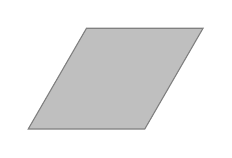
\begin{tikzpicture}[scale=0.37]            
        % \draw[help lines, color=black!30] (0,0) grid (16,16);
        \pavageLosange{15}{9};
        \coordinate (O) at (15,3*1.73);
        \tkzDrawPoint[shape=cross out, size=5pt](O);
        \tkzLabelPoints[above left](O);
        \coordinate (A) at (23,3*1.73);
        \coordinate (B) at (27,3*1.73);
        \coordinate (C) at (29,5*1.73);
        \coordinate (D) at (25,5*1.73);
        \draw[color=gray,fill=gray,fill opacity=0.5] (A) -- (B) -- (C) -- (D) -- cycle;
        % \imageHomothetyParallelogramme{0.5}{blue};
        % \imageHomothetyParallelogramme{1.5}{red};
        % \imageHomothetyParallelogramme{-1}{mygreen};
        % \imageHomothetyParallelogramme{-0.5}{black};
    \end{tikzpicture}
    \begin{enumerate}
        \item Colorier \textbf{en bleu} l'image de la figure grise par l'homothétie de centre $O$ et de rapport $\dfrac{1}{2}$.
        \item Colorier \textbf{en rouge} l'image de la figure grise par l'homothétie de centre $O$ et de rapport $\dfrac{3}{2}$.        
        \item Colorier \textbf{en vert} l'image de la figure grise par l'homothétie de centre $O$ et de rapport $-1$.        
        \item Colorier \textbf{en noir} l'image de la figure grise par l'homothétie de centre $O$ et de rapport $-\dfrac{1}{2}$.        
    \end{enumerate}
\end{exercice*}
\begin{corrige}
    %\setcounter{partie}{0} % Pour s'assurer que le compteur de \partie est à zéro dans les corrigés    
    \phantom{rrr}

    \hspace*{-5mm}
    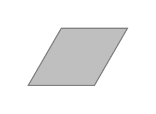
\begin{tikzpicture}[scale=0.21]            
        % \draw[help lines, color=black!30] (0,0) grid (16,16);
        \pavageLosange{15}{9};
        \coordinate (O) at (15,3*1.73);
        \tkzDrawPoint[shape=cross out, size=3pt](O);
        \tkzLabelPoints[above left](O);
        \coordinate (A) at (23,3*1.73);
        \coordinate (B) at (27,3*1.73);
        \coordinate (C) at (29,5*1.73);
        \coordinate (D) at (25,5*1.73);
        \draw[color=gray,fill=gray,fill opacity=0.5] (A) -- (B) -- (C) -- (D) -- cycle;

        \imageHomothetyParallelogramme{0.5}{blue};
        \imageHomothetyParallelogramme{1.5}{red};
        \imageHomothetyParallelogramme{-1}{mygreen};
        \imageHomothetyParallelogramme{-0.5}{black};
    \end{tikzpicture}

    \begin{enumerate}
        \item Colorier \textbf{en bleu} l'image de la figure grise par l'homothétie de centre $O$ et de rapport $\dfrac{1}{2}$.
        \item Colorier \textbf{en rouge} l'image de la figure grise par l'homothétie de centre $O$ et de rapport $\dfrac{3}{2}$.        
        \item Colorier \textbf{en vert} l'image de la figure grise par l'homothétie de centre $O$ et de rapport $-1$.        
        \item Colorier \textbf{en noir} l'image de la figure grise par l'homothétie de centre $O$ et de rapport $-\dfrac{1}{2}$.        
    \end{enumerate}
\end{corrige}

